\documentclass[a4paper]{article}

%% Language and font encodings
\usepackage[english]{babel}
\usepackage[utf8x]{inputenc}
\usepackage[T1]{fontenc}
\usepackage{graphicx}
\usepackage{float}       
%\usepackage{geometry}
\usepackage[left=4cm,right=3cm,top=3cm,bottom=2.5cm]{geometry}
\usepackage{vmargin}
\usepackage{fancyhdr}
\usepackage{epsfig}
\usepackage{eurosym}
\usepackage{url}
\graphicspath{ {figures/} }
\usepackage{array}
\usepackage{listings}
\usepackage{mathtools}

\newenvironment{Times}{\fontfamily{ptm}\selectfont}{}
\fancyhf{}
\pagestyle{fancy}
\fancyfoot[R]{\thepage}
\fancyhead[L]{\leftmark}
\usepackage{setspace}
\setstretch{1.5}

%Python code
\usepackage{listings}
\usepackage{color}

\definecolor{mygreen}{rgb}{0,0.6,0}
\definecolor{mygray}{rgb}{0.5,0.5,0.5}
\definecolor{mymauve}{rgb}{0.58,0,0.82}

\lstset{ %
  backgroundcolor=\color{white},   % choose the background color; you must add \usepackage{color} or \usepackage{xcolor}; should come as last argument
  basicstyle=\footnotesize,        % the size of the fonts that are used for the code
  breakatwhitespace=false,         % sets if automatic breaks should only happen at whitespace
  breaklines=true,                 % sets automatic line breaking
  captionpos=b,                    % sets the caption-position to bottom
  commentstyle=\color{mygreen},    % comment style
  deletekeywords={...},            % if you want to delete keywords from the given language
  escapeinside={\%*}{*)},          % if you want to add LaTeX within your code
  extendedchars=true,              % lets you use non-ASCII characters; for 8-bits encodings only, does not work with UTF-8
  frame=single,                    % adds a frame around the code
  keepspaces=true,                 % keeps spaces in text, useful for keeping indentation of code (possibly needs columns=flexible)
  keywordstyle=\color{blue},       % keyword style
  language=Python,                 % the language of the code
  morekeywords={*,...},            % if you want to add more keywords to the set
  numbers=left,                    % where to put the line-numbers; possible values are (none, left, right)
  numbersep=5pt,                   % how far the line-numbers are from the code
  numberstyle=\tiny\color{mygray}, % the style that is used for the line-numbers
  rulecolor=\color{black},         % if not set, the frame-color may be changed on line-breaks within not-black text (e.g. comments (green here))
  showspaces=false,                % show spaces everywhere adding particular underscores; it overrides 'showstringspaces'
  showstringspaces=false,          % underline spaces within strings only
  showtabs=false,                  % show tabs within strings adding particular underscores
  stepnumber=1,                    % the step between two line-numbers. If it's 1, each line will be numbered
  stringstyle=\color{mymauve},     % string literal style
  tabsize=2,                       % sets default tabsize to 2 spaces
  title=\lstname                   % show the filename of files included with \lstinputlisting; also try caption instead of title
}

\lstdefinestyle{customc}{
  belowcaptionskip=1\baselineskip,
  breaklines=true,
  frame=L,
  xleftmargin=\parindent,
  language=C,
  showstringspaces=false,
  basicstyle=\footnotesize\ttfamily,
  keywordstyle=\bfseries\color{green!40!black},
  commentstyle=\itshape\color{purple!40!black},
  identifierstyle=\color{blue},
  stringstyle=\color{orange},
}

\lstdefinestyle{customasm}{
  belowcaptionskip=1\baselineskip,
  frame=L,
  xleftmargin=\parindent,
  language=[x86masm]Assembler,
  basicstyle=\footnotesize\ttfamily,
  commentstyle=\itshape\color{purple!40!black},
}

\title{\underline{\textbf{\begin{Huge}Network\end{Huge}}}\\\vspace{1cm}
    \begin{huge}
        \textbf{Client / Server communication study}
    \end{huge}\\}
    
\author{
        Tom Moulard (16920041)
        \date{}
        }
        
        
\begin{document}
\maketitle
\begin{center}
\vspace{1cm}
\date{2017 June 15}
\vspace{2cm}\\
\end{center}    
    \thispagestyle{empty}

\newpage{}

\tableofcontents
\thispagestyle{empty}

\newpage
\section{Introduction}

When studying the operation of the exchanges between two computers, the best way to understand it is to see what they are actually saying to each others.
I thus created a small Python Program to make two computer communicate, one as a server and the other as a client sending a file to the server.
We are going to see how this program works in details and how the computers have managed to talk to each other in order to send this file.  

\section{Code}

\subsection{Actual code}
\lstinputlisting[language=Python]{customIperf.py}

\subsection{Explanations}
%This section should explain how the code works

This code initiates the connection between two computers and allows one to send a file to the other.
Indeed, in order to proceed, we need to have two computers able to interpret a python code.
We also need to indicate which one is going to be the server and with one the client.
Once it is done, we have to run the interpreter in a terminal following this method : \textit{python3 customIperf.py -s} for the server.\\
The client computer requires some more datas, you need to know the IP address of the server.Wether it is Internal or external, that is up to you to choose, depending on how these two computers can communicate together. Afterwards you can run this : \textit{python3 customIperf.py -c <Server IP address> <file>}. The file can be every file on you computer, it will e stored on the server with the same name.

When running the code, the first thing is to need to indicate the role of the computer : \textit{-s} for server, \textit{-c} for client.

\subsubsection*{Server}

Once the computer knows that it is going to be the server it will open the setted port to allow clients to connect to him. To set the port, you can either choose a random setting, or do it manually. Then the server will wait for a client signal to establish the connection.\\
When a client tries to connect to the server, informations will be gathered by the server about the client to be able to communicate with him.\\
 Once it is done, the server will wait to receive a number which correspond of the length of the fileName. Then it will observe the fileName using it's length and will create a new file with this fileName.\\
After that the document has been created, the server will gather all informations going through the network buffer to watch rights packets to add to the file. When the server sees a EOF signal, it closes the document and ends the connection with the client.
Now another client can connect to the server in order to send another file.

\begin{figure}[H]
\centering
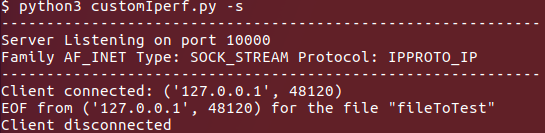
\includegraphics[width=0.6\textwidth]{serverSide.png}
\caption{Server side output}
\end{figure}

\subsubsection*{client}

The client is quite the opposite of the server.\\
The client is going to try to establish the connection with the ip/port given by the user to the server. If nothing is founded, the client will just wait for the server to be started.\\
When the connection is established, it will send the length of the fileName, the fileName and then the document.

\begin{figure}[H]
\centering
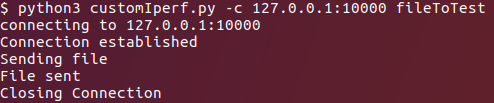
\includegraphics[width=0.6\textwidth]{clientSide.png}
\caption{Client side output}
\end{figure}

Also, as you can notice, I made this code an only file to make it easier to use. %one script to rule them all
It makes it easier to transmit between computers and easier to change from client to server or from server to client.

In case there is an issue with the connection, python will throw an exception to tell the user what happened to help him correct the mistakes. But the only weakness of my script is when transferring a file, if something is wrong, it won't be able to detect the issue and the output file located on the server might be corrupted.

Which lead us to possibles improvement that can be done for this script.
In fact, this is the base of the process of advanced and stylish file transfer like emails, WWW(World Wide Web), FTP(File Transfer Protocol), or even streaming data for instance.
So there is a lot of ways to improve this script, but it depends on the usage/main characteristics we want it to have like security, compression, effectiveness, ...

\newpage
\section{Interpretation}
%This looks at wireshark screens and explain what the f*** appended

Now that the easy part has been completed, we can focus more deeply on what is really important here: the network.

\begin{figure}[H]
\centering
\includegraphics[width=1\textwidth]{WS_-_General_lookup.png}
\caption{Wireshark output}
\end{figure}

This is showing the main display of Wireshark for this file sharing, where we can notice the different ports.
Since i am running both the client and the server from my computer they all have the same ip, but only the port changes : 10000 for the server and 56158 for the client.\\
Just by looking at an overview of it, we can see three distinct part: The Authentication Part (or the Connection Establishment Part), The Data Transfer Part and The Close connection Part. Each following a natural flow, the authentication first, the data transfer in second and then the connection. 

\subsection{The Authentication Part}

As we can see in the column Protocol, this connection was established in TCP which means that the authentication part was managed by a three way handshake protocol.

\subsubsection{The (famous) Three Way Handshake}

This protocol is implemented in three phases : the Synchronize(SYN) message, synchronize-Acknowledgment(SYN-ACK) message and the Acknowledgment(ACK) message. This protocol ensure that both client and server are synchronized and that they are ready to communicate.

\subsubsection{The Synchronize Message}

This message is send by the client to ask the server if he is available for a new client connection.
In our case, it is the first packet on the list with the info beginning by "[SYN]" and we can see the port source is the client and the port destination is the server.
We can also notice the the Seq=0 which means that it is the first packet of this discussion.

\subsubsection{The Synchronize - Acknowledgment Message}

This is the response from the server to the client, as we can see on the source and destination port and on the flags : "[SYN - ACK]".
We can observe that the flag Seq is also null showing that it is the server's own sequence but the ACK number is 1 which means that the server received the first packet.

\subsubsection{The Acknowledgment Message}

This is the final packet send / received for the Handshake. This packet (n°3 here) have an ACK number at 1 (SEQ from the packet n°2 + 1) and the server does not need to reply for this one knowing that both client and server are ready to discuss.

\subsection{The Data Transfer Part}

After the communication has been established and an authentication performed, the actual data transfer can begin.
In my code, I specified that the length of the fileName should be less than 10\^512 and therefore the first packet the program send is a packet with a length of 580 : 512 of data ("len=512") and 68 of header. 
The fileName of the file I sent is equal to "fileToTest" and has a length of 10 characters.
Also, we can note that the ACK number follows the SEQ number of the previous packet.
\\
Then the server replies with another packet, with a SEQ number following the last ACK one, to tell the client that it has received the packet and that he have a good checksum, so there is no data loss.
\\
After this, my program sends the fileName encoded in UTF-8 in another packet. And the server replies that he received the packet and everything works right. Since the fileName has a length of 10, the server is waiting to receive a packet with a data of this length and the "len=10" characteristic can attest this. 
\\
To finish the data sending, the program sends the content of the file. the server will just receive all packet from this client and append them to the file.

\subsection{The Close Connection Part}

To properly end the connection, the client sends a "FIN" packet to tell the server to close the connection and the file.
\\
The server simply respond that he got all packet and that he will close the connection.

\section{Conclusion}

Now we can understand how theses communication occurred to transmit a file between two computers using a TCP connection.

\newpage
\listoffigures
\end{document}